% \documentclass{article}
\documentclass{foresj}
\usepackage[utf8]{inputenc}
\usepackage{graphicx}
\usepackage{booktabs}
%\usepackage[binary-units]{siunitx}
%\usepackage[running]{lineno}
%\usepackage[]{authblk} % options: affil-it
%\usepackage{setspace}
%\usepackage{natbib}
\usepackage{amsmath}
\usepackage{amssymb}
\usepackage{bm}
%\usepackage{hyperref}
%\usepackage{verbatim}

\DOI{0000000}
\Year{2019}

\begin{document}

\title{A simplified method for estimating stem diameter distributions from horizontal point sample data}

\author[Paradis, GE]{Gregory E Paradis$^{\ast}$}
% \affiliation{$^1$ Department of Forest Resources Management,  University of British Columbia, Vancouver, BC, Canada.}
\corres{$^{\ast}$Corresponding author. Department of Forest Resources Management,  University of British
  Columbia. \texttt{gregory.paradis@ubc.ca}}
\date{\rec{4 September 2019}}

\begin{abstract}
Horizontal point sampling (HPS) is a common forest inventory technique. 
When HPS tally data is expanded into stand table format, estimation error on stem density is size-biased and proportional to expansion factors. 
The size-biased nature of HPS data must be accounted for when estimating stem diameter distributions, otherwise the distribution parameters will be over-fitted to data points in small diameter classes. 
One way to account for this is to fit special size-biased forms of common statistical distributions to raw (unexpanded) HPS tally data. 
We describe an alternative method, which involves fitting standard distribution forms to expanded HPS tally data with the size bias implemented in the fitting algorithm. 
The main advantage of our alternative method is that it can be
implemented easily using existing probability distribution functions
and parameter-fitting algorithms built
into statistical software libraries.
This obviates the need for analysts to derive special size-biased
distribution forms, and helps improve parameter-fitting algorithm stability. 
We ran a computational experiment comparing output of reference and
alternative methods, and show that output from our alternative method
is essentially identical to output from the reference method. 
Given the functional equivalence of our alternative method (and its
improved simplicity and stability), we recommend that our method be
used for practical applications.
\end{abstract}

\maketitle

%\linenumbers 
%\doublespace 

\section{Introduction}
\label{sec:introduction}

Horizontal point sampling (HPS), also known as Bitterlich \citep{bitterlich1947winkelzahlmessung} or prism sampling, is a common forest inventory technique. 
\emph{Stem density} refers to the number of stems per unit area (e.g.,
stems per hectare) in a given stand. 
A \emph{stand table} is essentially a vector $\bm{\hat{Y}} = (\hat{y}_1, \hat{y}_2... , \hat{y}_{|I|})$ of mean stem density estimates, binned by diameter at breast height (DBH) size class $i \in I$. 
Stem density $\hat{y}_i$ in size class $i \in I$ compiled from a set $J$ of HPS sample plots, inventoried using a prism with basal area factor $C_B$, is given by

\begin{equation}
\hat{y}_i = C_B \sum_{j \in J} t_{ij}\left(\bar{g}_{ij}|J|\right)^{-1}, \quad \forall i \in I
\end{equation}

where $\bar{g}_{ij}$ denotes mean basal area of the $t_{ij}$ stems in size class $i$ in plot $j$.

Assuming that variance of binned tally frequency data is homogeneous with respect to $i$, variance of stem density estimates will be heteroscedastic, proportional to $C_B\bar{g}_{ij}^{-1}$. 
Thus, we can describe estimation error on $\bm{\hat{Y}}$ as \emph{size-biased}.

It can be useful to fit empirical data to well-known statistical
distributions, for example to implement inverse transform sampling \citep{devroye1986nonuniform} in
a simulation model. 
Applying standard distribution-fitting techniques to expanded (stand
table) HPS data in $\bm{\hat{Y}}$ is incorrect, and results in
over-fitting the model to data in small diameter size classes.
This problem can be overcome by fitting a size-biased form of the
assumed distribution to the raw (unexpanded) HPS tally data. 

The use of size-biased distributions for fitting assumed diameter
distributions to HPS tally data was first described in
\citet{vandeusen1986fitting}.
\citet{gove2000some} points out that scarcity of published
work on fitting size-biased assumed distributions to HPS tally data is at odds with
the potential value of this type of model, given abundance and
availability of HPS tally data collected from managed forest stands.

\citet{ducey2015sizebiased} describe size-biased forms of several statistical distributions that can be used to fit raw (unexpanded) HPS tally data.
They show that fitting size-biased distributions to HPS tally data
produces better results, compared to fitting standard distributions to
stand table data.
In the same paper, the authors also document size-biased forms for a
number of distributions in the generalized beta family.
Deriving size-biased forms for other distributions is not trivial and
may in some cases be very difficult or impossible. 
Furthermore, these size-biased forms are not implemented in most common statistical software packages. 
Before the method described in \citet{ducey2015sizebiased} can be applied, the size-biased distribution forms may need to be algebraically derived (or
extracted from previously published work) and subsequently implemented within the software environment
used for distribution fitting.
This necessary step of deriving and
implementing the size-biased forms of assumed distributions may represent a
non-trivial technical challenge for less experienced analysts and
forest practitionners.

We developed an alternative method for fitting diameter distributions
to expanded HPS data, using standard forms of statistical
distributions and a weighted residuals vector in the non-linear
least squares (NLLS) fitting algorithm.
Our alternative method is mathematically equivalent to the method
described in \citet{ducey2015sizebiased} but avoids the need to
derive and implement special size-biased forms of the target
distributions.
Furthermore, parameter bound constraints for the standard-form
distributions used in our alternative method are arithmetically
simpler, so our method should be more stable in practice (i.e., require less expert parameter-tweaking
of the NLLS algorithm to yield acceptable results).

We present results from a computational experiment, where we compare
output from alternative and reference methods.
We fit stem diameter data from three metaplots (compiled from sample plot
data collected in Quebec, Canada), to both Weilbull and gamma
distributions. We use a bin-wise residual sum of squares (RSS)
statistic to report similarity of output from both methods.

\section{Methods}
\label{sec:methods}

We describe a computational experiment that compares output from
alternate (henceforth referred to as \emph{test}) and reference
(henceforth referred to as \emph{control}) parameter-fitting methods. 
We fit both Weibull and gamma distributions using control
and test methods to empirical stem
diameter data from three meta-plots, for a total of six replicates.

Our experimental dataset is extracted from a database of permanent sample plot (PSP) data
collected throughout Quebec, Canada \citep{quebec2018pep}.
The dataset is freely available from \emph{Le carrefour
  collaboratif en données ouvertes québécoises}\footnote{Detailed
  information on the Quebec
  PSP inventory program under which our test data was collected is
  available from the Ministère des forêts, faune, et parcs (MFFP) web site
  (\url{http://mffp.gouv.qc.ca/les-forets/inventaire-ecoforestier/}), including
  technical documentation on inventory methods, data standards, and
  contact information. The full PSP dataset can be downloaded from \url{https://www.donneesquebec.ca}.}.
The full dataset consists of over 1 million stem measurements,
collected from over 12000 plots split across 8 plot networks, with
repeated measures on a 10-year inventory cycle.
For the purposes of our experiment, we extracted a subset of stems in this dataset to
include only live, merchantable stems from the fourth decennial inventory
cycle, from the largest of 8 plot networks, corresponding to mature, undisturbed stands, for which there was valid
data in all fields.
The full procedure for extracting our experimental dataset from the
full PSP dataset is described in a Jupyter notebook, including Python
code for replicating the procedure from
source data---the notebook can be downloaded from GitHub\footnote{\url{https://www.github.com/hpsdistfit}}.

The filtered dataset consists of 52~192 stems, collected from 11.28 m
radius circular fixed-area plots.
We chose this dataset because we did not have access to a comparable
database of HPS inventory data at the time we ran the computational
experiment. We manipulated the PSP tally data to emulate an HPS dataset.
PSP tally data has a constant expansion factor for all stems, so the empirical diameter distribution of PSP tally data has the same shape as the expanded (stand table) empirical diameter distribution. 
For the purposes of our experiment, we simply assume that the expanded PSP tally data corresponds to expanded HPS tally data. 
We simulate binned HPS tally data by scaling the expanded binned PSP data by $g_i^{-1}$, which corresponds to reciprocal of the HPS expansion factor, assuming $C_B = 1$. 
This manipulation of expanded PSP data will adequately simulate HPS
tally data for the purpose of our experiment, if we assume that stem density estimation error is proportional is proportional to $g_i^{-1}$.

The control method fits size-biased forms of Weilbull and gamma
distributions to the binned and normalized meta-plot data (compressed to simulate HPS tally data), using an unweighted objective function in the fitting algorithm.
The test method fits Weibull and gamma distributions to the binned and
normalized meta-plot data (expanded to stand table form), using a weighted objective function in the fitting algorithm.
All other parameters are held constant for both methods.

%of $C_Bg_i^{-1}$ to calculate the residuals for all size classes in the objective function of the fitting algorithm, with $g_I$ corresponding to the basal area of a stem with diameter centered on upper and lower bounds of size class $i$.

Both test and control methods use the same weighted non-linear least
squares (NLLS) algorithm
 \footnote{Our software implementation of the
   computational experiment described here uses the \texttt{scipy.optimize.curve\_fit}
   function from the commonly used SciPy open source Python software
   package (see \url{https://scipy.org/}), which implements several NLLS
   algorithms that can be used to model fit parameters to empirical
   data. We pass a vector of bin-wise HPS expansion factor values as
   the the optional \texttt{sigma} argument to
   \texttt{curve\_fit}, which reduces the relative weight of smaller
   diameter classes in the NLLS algorithm.}
to fit assumed distribution parameters to inventory data binned into
diameter size classes of uniform width $W$.
The objective function value of the NLLS problem minimizes the sum of
squares of the residual terms

\begin{equation}
Z = \text{min} \quad \sum_{i \in I} e_i^2
\end{equation}

    with

   \begin{equation}
    e_i := e\left(f(x_i; \bm{P}), \hat{y}_i\right) = w_i \left[f(x_i; \bm{P}) - \hat{y}_i\right] 
  \end{equation}
  
  where $x_i$ is the diameter corresponding to the center of bin $i
  \in I$, $f(x_i; \bm{P})$ is the value of the probability
  distribution function (PDF) at $x_i \in \bm{X}$ (given a vector of
  parameters $\bm{P}$), $\hat{y}_i \in \bm{\hat{Y}}$ represents the
  estimated stem density in bin $i$ (stem tally for the control method, stem density for the test method), and $w_i$ is the weight associated with bin $i$ (1 for the control method, $g_i^{-1}$ for the test method).

Data from each meta-plot was fit to both two-parameter Weibull (W) and
two-parameter gamma (GA) distributions, which have often been used to model stem diameter \citep{bailey1973quantifying, cao2004predicting, ducey2015sizebiased, zutter1986characterizing, hafley1977statistical}.
Both Weibull $f_W(x; a, b)$ and gamma $f_{GA}(x; b, p)$ distributions are
special cases of the three-parameter generalized gamma (GG)
distribution  $f_{GG}(x; a, b, p)$, which has the the following form

\begin{equation}
f_{GG}(x; a, b, p) = \frac{ax^{ap-1}e^{-\left(\frac{x}{b}\right)^a}}{b^{ap}\Gamma(p)}, \qquad a > 0, b > 0, q > 0
\end{equation}

defined for $x > 0$, where $\Gamma(p)$ represents the gamma function (not to be confounded with the gamma distribution), which is given by

\begin{equation}
\Gamma(p) = \int_0^\infty x^{p-1}e^{-x} dx.
\end{equation}


The size-biased form of $f_{\text{GG}}(x; a, b, p)$ is given by 

\begin{align}
f^{\text{SB}}_{\text{GG}}(x; a, b, p, \alpha) &= f_{\text{GG}}(x;
                                                    a, b, p +
                                                    \alpha/a) & \alpha
                                                                > -ap
\end{align}

where $\alpha$ corresponds to the \emph{order} of the distribution (adapted from \citealp{ducey2015sizebiased}).
For the case of HPS, which is an area-based sampling technique, we

need a size-biased distribution of order 2 as basal area is related to
the square of diameter.
Thus, we set $\alpha=2$ for all size-biased distribution fitting in the control scenario (i.e., this parameter is fixed, and is not fit by the NLLS algorithm).

%Data from each meta-plot was fit to both two-parameter Weibull and two-parametr gamma distributions, which have been used to characterize stem diameters in forest stands \citep{bailey1973quantifying, cao2004predicting, ducey2015sizebiased, zutter1986characterizing, hafley1977statistical}.
%Both Weibull $f_{\text{W}}(x;a, \beta)$ and gamma $f_{\text{GA}}(x; \beta, p)$ distributions are special cases of the three-parameter generalized gamma distribution $f_{\text{GG}}(x; a, \beta, p)$.

We can define both standard and size-biased forms
of Weibull and gamma distribution PDFs in terms of the GG distribution
PDFs.
The standard forms are given by

%{\small

  \begin{align}
f_{\text{W}}(x; a, b) &= f_{\text{GG}}(x; a, b, 1), & a > 0, b > 0 \\
f_{\text{GA}}(x; b, p) &= f_{\text{GG}}(x; 1, b, p), & b > 0, p > 0
\end{align}
%}%

and the size-biased forms are given by (adapted from \citealp{ducey2015sizebiased})

%{\small
\begin{align}
f^{\text{SB}}_{\text{W}}(x; a, b, \alpha) &= f^{\text{SB}}_{\text{GG}}(x; a, b, 1 + \alpha/a),& a > 0, b > 0, \alpha > -a \\
f^{\text{SB}}_{\text{GA}}(x; b, p, \alpha) &= f^{\text{SB}}_{\text{GG}}(x; 1, b, p + \alpha),& b > 0, p > 0, \alpha > -p 
\end{align}
%}%

We segmented our experimental dataset into 30 meta-plots (combinations
of 10 species groups and 3 cover types).
We ran the computational
experiment on three of these meta-plots, corresponding to
spruce-pine-fir-larch (SPFL) in softwood stands (SPFL-S), white birch
in mixedwood stands (birch-M), and sugar maple in hardwood stands
(maple-H).
For each combination of meta-plot and assumed distribution, we report
an RSS statistic that measures the difference between the best-fit
PDFs output from  control and test methods.
Specifically, the RSS statistic corresponds to the sum of bin-wise squared differences
between a vector of pairs of points corresponding to PDF function
value at bin-wise centers, for control and test best-fit
PDFs.
For a given meta-plot and assumed distribution, the RSS statistic is
given by

\begin{equation}
  \text{RSS} = \sum_{i \in I}\left[g_i f_C(x_i; \bm{P}_C) - f_T(x_i; \bm{P}_T)  \right], \quad \forall i \in I
\end{equation}

where $f_C(x_i; \bm{P}_C)$ and $f_T(x_i; \bm{P}_T)$ represent best-fit
PDFs from control and test methods.
Note that $f_C$ must be projected into stand table space using
bin-wise expansion factor $g_i$ for comparison with $f_T$. 
The experiment tests the hypothesis that $f_C$ and $f_T$ are
equivalent. 

\section{Results}
\label{sec:results}

Figure \ref{fig:results} compares best-fit distributions for control
and test methods (shown with dashed and solid lines, respectively) against empirical input data distribution (shown with gray circles), binned by
diameter class.
  Subfigure rows correspond to meta-plots (i.e., SPFL-S, birch-M, maple-H).
  Sufigure columns correspond to target distributions (i.e., Weibull, gamma).
  Table \ref{tab:results} shows sample size and RSS statistic for each
  replicate (combinations of meta-plot and target distribution). 

  Visual inspection of the best-fit PDFs in Figure \ref{fig:results}
  confirms that control and test methods yield virtually identical
  results for all six replicates.
  This observation is supported by small RSS values in Table
  \ref{tab:results}.
  These results empirically confirm our hypothesis that control and
  test methods are functionally equivalent, for all six replicates in
  our computational experiment.

  [Figure \ref{fig:results} goes here.]
  
  [Table \ref{tab:results} goes here.]


\section{Discussion}
\label{sec:discussion}

The control method in our computational experiment implements the reference method described in
\citet{ducey2015sizebiased}---it fits a special size-biased form of the target distribution to raw (tally) HPS data. 
In contrast, the test method in our computational experiment
implements our alternative method---it uses the standard form of the target
distribution and a vector of (easily computed) expansion factor values
to weight the least-squares fit algorithm.
Computational experiment results confirm the hypothesis that control and
test methods are functionally equivalent. 
Thus, the test method constitutes a valid replacement for the control
method.

In contrast with the control method, the test method does not
require algebraic derivation of special size-biased distribution
functions, or implementation of these special functions in the software environment used
for analysis.
Validity conditions for standard forms of distributions can usually be expressed in terms of upper and lower bounds on parameter values. 
In contrast, validity conditions for the size-biased forms of the same distributions are more complex, with parameter bounds  involving algebraic expressions of other parameters. 
If the best fit value of a parameter is very close to a constraint boundary, the derivative estimated uncertainty and correlations for that parameter (which are typically estimated using some form of numerical approximation implemented in the fitting algorithm) may not be reliable.
Effort required to tweak fitting algorithm parameters to produce acceptable results (in particular with respect to estimated parameter uncertainty and correlations) is proportional to the complexity of constraints required to ensure validity conditions of the target distribution are respected.
Thus our alternative method, which uses less constrained standard
forms of distributions, should be less susceptible to computational
tractability issues in practice.

Given that the test method is simpler to apply and potentially more
stable than the control method (while yielding equivalent output), we
recommend its use in practical applications.

Based on our experimental results, we conjecture that our test method will be
functionally equivalent to the control method for any inventory
dataset---empirically testing the limitations of this conjecture on new
datasets constitutes a potential direction for further research.
We have not presented a theoretical proof of equivalence of control
and test methods, however development of such a proof would would
strengthen our conjecture and represents another interesting opportunity for further research.

To facilitate application of our method, we provide a Jupyter Notebook
containing instructions and code that can be used to
reproduce our computational experiment, as well as constitute a
known-working software implementation of our method (which can provide
a good starting point for further research or application of our method to other contexts).

\section{Conclusion}
\label{sec:conclusion}

  In this paper we presented a new method for deriving stem diameter
  distributions from HPS tally data.
  Using a computational experiment, we compared output of our new
  method to the reference method (which uses special size biased forms
  of target distribution PDFs), and showed that performance of our new
  method is essentially identical (i.e., yields the same shape
  best-fit curves for six combinations of species group, cover
  type, and target distribution).
  Advantages of our method include improved simplicity of application (i.e.,
  uses standard PDF forms instead of requiring algebraic derivation of
  special size-biased forms, and uses readily-available fitting
  functions built into common data analysis software packages), and improved stability
  (i.e., requires less software parameter tweaking to yield acceptable
  results).

  In summary, based on our observation that our new method has no
  obvious down-sides and presents some clear advantages, we recommend
  its use in practical applications. 

  Consistently with the principles of FAIR\footnote{Findable,
    Accessible, Interoperable, Reusable.} science
  \citep{stall2019make, wilkinson2016fair}, we implemented our
  experiment in a Jupyter Notebook using open-source Python libraries,
  which is available for download from a public GitHub
  repository\footnote{https://github.com/gparadis/hpsdistfit}.
  
  \section*{Funding}

This study was supported by funding from the \emph{FORAC Research
  Consortium}; \emph{Genome BC}; and \emph{Genome Quebec}.

\section*{Acknowledgements}

The author thanks Adam Polinko and Valerie Lemay for their valuable comments and
suggestions on an earlier drafts of the work presented here.


%\begin{nolinenumbers}
%%\bibliographystyle{apalike}
%\bibliographystyle{foresj}
%%\nocite{*} % adds all references in the bib file to the bibliography (cited or not)
%\bibliography{refs.bib}
%\end{nolinenumbers}

\clearpage

\begin{thebibliography}

\bibitem[Bailey and Dell(1973)]{bailey1973quantifying}
Bailey, RobertL and Dell, TR 1973 Quantifying diameter distributions with the
  weibull function.
\textit{Forest Science} \textbf{19}, 97--104.

\bibitem[Bitterlich(1947)]{bitterlich1947winkelzahlmessung}
Bitterlich, Walter 1947 Die winkelzahlmessung.
\textit{Allegemeine Forst-und Holzwirtschaftliche Zeitung} \textbf{58}, 94--96.

\bibitem[Cao(2004)]{cao2004predicting}
Cao, QuangV 2004 Predicting parameters of a weibull function for modeling
  diameter distribution.
\textit{Forest science} \textbf{50}, 682--685.

\bibitem[Devroye(1986)]{devroye1986nonuniform}
Devroye, Luc 1986 \textit{{Non-Uniform Random Variate Generation}}.
New York: {Springer-Verlag}.

\bibitem[Ducey and Gove(2015)]{ducey2015sizebiased}
Ducey, MarkJ and Gove, JeffreyH 2015 Size-biased distributions in the
  generalized beta distribution family, with applications to forestry.
\textit{Forestry} \textbf{88}, 143--151.

\bibitem[{Gouvernement du Québec}(2019)]{quebec2018pep}
{Gouvernement du Québec} 2019 {Placettes-échantillons permanentes}.
available at \url{https://www.donneesquebec.ca}.

\bibitem[Gove(2000)]{gove2000some}
Gove, JeffreyH 2000 Some observations on fitting assumed diameter distributions
  to horizontal point sampling data.
\textit{Canadian journal of forest research} \textbf{30}, 521--533.

\bibitem[Hafley and Schreuder(1977)]{hafley1977statistical}
Hafley, WL and Schreuder, HT 1977 Statistical distributions for fitting
  diameter and height data in even-aged stands.
\textit{Canadian Journal of Forest Research} \textbf{7}, 481--487.

\bibitem[Stall et~al.(2019)]{stall2019make}
Stall, Shelley, Yarmey, Lynn, Cutcher-Gershenfeld, Joel, Hanson, Brooks,
  Lehnert, Kerstin, Nosek, Brian, Parsons, Mark, Robinson, Erin and Wyborn,
  Lesley 2019 Make scientific data fair.

\bibitem[Van~Deusen(1986)]{vandeusen1986fitting}
Van~Deusen, PaulC 1986 Fitting assumed distributions to horizontal point sample
  diameters.
\textit{Forest Science} \textbf{32}, 146--148.

\bibitem[Wilkinson et~al.(2016)]{wilkinson2016fair}
Wilkinson, MarkD, Dumontier, Michel, Aalbersberg, IJsbrandJan, Appleton,
  Gabrielle, Axton, Myles, Baak, Arie, Blomberg, Niklas, Boiten, JanWillem,
  da~Silva~Santos, LuizBonino, Bourne, PhilipE et~al. 2016 The fair guiding
  principles for scientific data management and stewardship.
\textit{Scientific data} \textbf{3}.

\bibitem[Zutter et~al.(1986)]{zutter1986characterizing}
Zutter, BR, Oderwald, RG, Murphy, PA and Farrar~Jr, RM 1986 Characterizing
  diameter distributions with modified data types and forms of the weibull
  distribution.
\textit{Forest Science} \textbf{32}, 37--48.

\end{thebibliography}




\clearpage

\begin{figure}[h!]
  \centering
  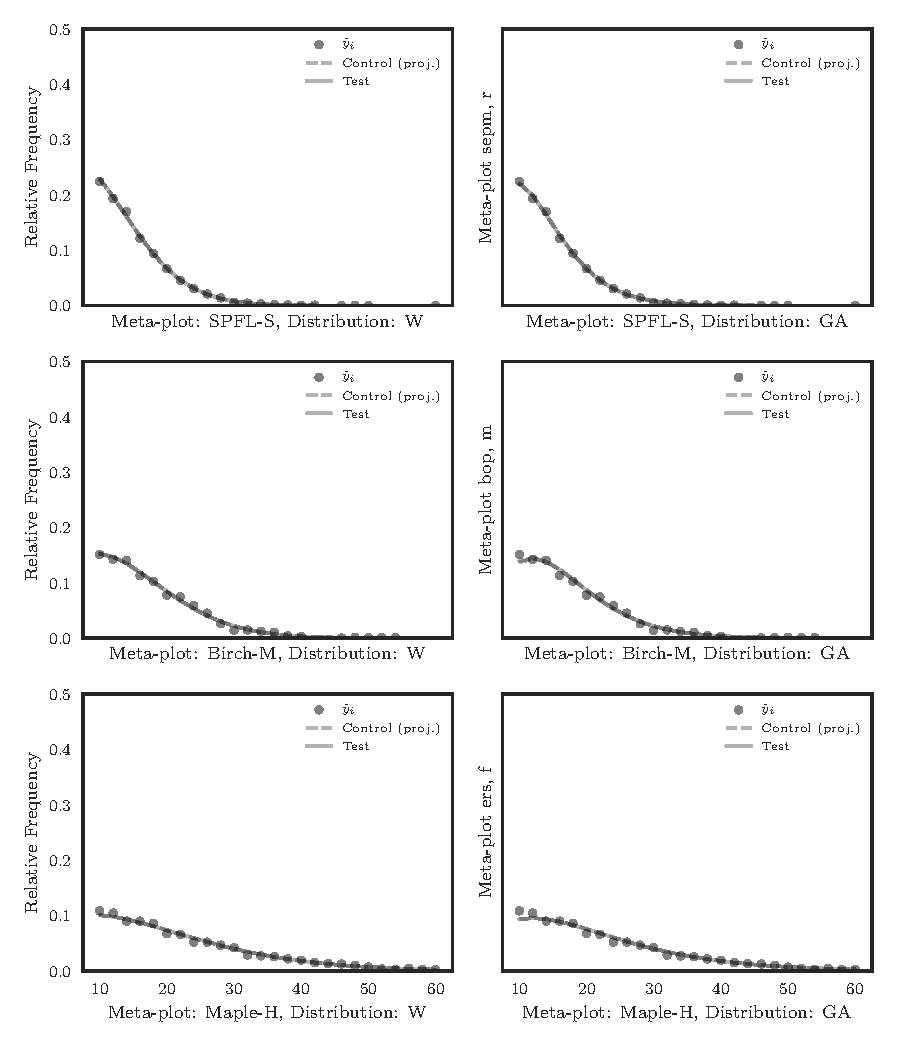
\includegraphics[width=1.0\textwidth]{results}
  \caption{Best-fit distributions for control (solid black line) and test (dotted black line) scenarios. Empirical distribution of expanded (stand table) sample data is shown with gray circles, binned by diameter class. Distributions from the control scenario are projected onto expanded data space.}
  \label{fig:results}
\end{figure}

\begin{table}[h!]
\caption{Sample size and residual sum of squares (RSS) statistic, by meta-plot
  (species group and cover type) and distribution. RSS is computed from bin-wise difference between test and control best-fit distributions.}
\vspace{1em}
\label{tab:results}
\centering
\begin{tabular}{lllrr}
\toprule
  Species & Cover Type & Distribution &  Sample Size &           RSS \\
  \midrule
  SPFL &   Softwood &  W &       6115 &  1.82 $\times 10^{-09}$ \\
  SPFL &   Softwood &  GA &       6115 &  1.31 $\times 10^{-10}$ \\
  Birch &  Mixedwood &   W &      1605 &  5.85 $\times 10^{-08}$ \\
  Birch &  Mixedwood &     GA &    1605 &  8.08 $\times 10^{-06}$  \\
  Maple &   Hardwood &      W &   1290 &  1.60 $\times 10^{-09}$ \\
  Maple &   Hardwood &      GA &   1290 &  5.35 $\times 10^{-09}$ \\
\bottomrule
\end{tabular}
\end{table}


\end{document}


%%% Local Variables:
%%% mode: latex
%%% TeX-master: t
%%% End: